\section{Geometric interpretation of linear transformations}

\begin{outcome}
  \begin{enumerate}
  \item Find the matrix of rotations, reflections, scalings, and
    shearings in $\R^2$ and $\R^3$.
  \item Determine the action of a rotation or reflection on a vector.
  \end{enumerate}
\end{outcome}

In this section, we will examine some special examples of linear
transformations in $\R^2$ and $\R^3$ including rotations and
reflections.

\begin{example}{Rotation by $90^{\circ}$ in $\R^2$}{rotation-90-R2}
  Consider the linear transformation $T:\R^2\to\R^2$ that is given by
  a counterclockwise rotation by 90 degrees. Find the matrix%
  \index{matrix!of a rotation}%
  \index{rotation!matrix of}%
  \index{linear transformation!rotation} $A$ corresponding to this
  linear transformation. Find a formula for $T$.
\end{example}

\begin{solution}
  To visualize a vector function on $\R^2$, it is often useful to
  consider a pair of before-and-after pictures such as the following:
  \begin{center}
    \begin{tikzpicture}
      \begin{scope}[scale=0.5]
        \draw[red,thick,fill=red!10]
        (0,0) -- (0,5) -- (3,5) -- (3,4) -- (1,4) --
        (1,3) -- (2,3) -- (2,2) -- (1,2) -- (1,0) -- cycle;
        \draw[step=1cm, gray!50, very thin] (-5.8,-5.8) grid (5.8,5.8);
        \draw[thick,->] (-6.5,0) -- (6.5,0);
        \draw[thick,->] (0,-6.5) -- (0,6.5);
        \draw[red,thick]
        (0,0) -- (0,5) -- (3,5) -- (3,4) -- (1,4) --
        (1,3) -- (2,3) -- (2,2) -- (1,2) -- (1,0) -- cycle;
        \draw[blue,thick,->] (0,0) -- node[below] {$\vect{e}_1$} (5,0);
        \draw[blue,thick,->] (0,0) -- node[left] {$\vect{e}_2$} (0,5);
        \path (0,-7.2) node {``before''};
      \end{scope}
      \begin{scope}[xshift=4.5cm]
        \path (0,0) node {$\stackrel{T}{\longmapsto}$};
      \end{scope}
      \begin{scope}[xshift=9cm,scale=0.5]
        \draw[red,thick,fill=red!15,rotate=90]
        (0,0) -- (0,5) -- (3,5) -- (3,4) -- (1,4) --
        (1,3) -- (2,3) -- (2,2) -- (1,2) -- (1,0) -- cycle;
        \draw[step=1cm, gray!50, very thin] (-5.8,-5.8) grid (5.8,5.8);
        \draw[thick,->] (-6.5,0) -- (6.5,0);
        \draw[thick,->] (0,-6.5) -- (0,6.5);
        \draw[red,thick,rotate=90]
        (0,0) -- (0,5) -- (3,5) -- (3,4) -- (1,4) --
        (1,3) -- (2,3) -- (2,2) -- (1,2) -- (1,0) -- cycle;
        \draw[blue,thick,->,rotate=90] (0,0) -- node[right]
        {$T(\vect{e}_1) = \begin{mysmallmatrix}{c}0\\1\end{mysmallmatrix}$}
        (5,0);
        \draw[blue,thick,->,rotate=90] (0,0) --
        node[below,xshift=-0.1cm] {$T(\vect{e}_2) = \begin{mysmallmatrix}{c}-1\\0\end{mysmallmatrix}$}
        (0,5);
        \path (0,-7) node {``after''};
      \end{scope}
    \end{tikzpicture}
  \end{center}
  The picture illustrates how the function $T$ rotates the entire
  plane (including the pink letter ``F'') by 90 degrees
  counterclockwise. The picture also illustrates that when we apply
  the rotation $T$ to the first and second standard basis vectors
  $\vect{e}_1$ and $\vect{e}_2$, we obtain the vectors
  \begin{equation*}
    T(\vect{e}_1) = \begin{mymatrix}{c}0\\1\end{mymatrix}
    \quad\mbox{and}\quad
    T(\vect{e}_2) = \begin{mymatrix}{c}-1\\0\end{mymatrix}.
  \end{equation*}
  The matrix of $T$ has these vectors as its columns. Therefore, the
  matrix of $T$ is
  \begin{equation*}
    A = \begin{mymatrix}{cc}
      0 & -1 \\
      1 & 0 \\
    \end{mymatrix}.
  \end{equation*}
  Finally, we can use this to find a formula for the counterclockwise
  90 degree rotation $T$:
  \begin{equation*}
    T\tup{\begin{mymatrix}{c} x \\ y \end{mymatrix}}
    = \begin{mymatrix}{cc}
      0 & -1 \\
      1 & 0 \\
    \end{mymatrix}
    \begin{mymatrix}{c} x \\ y \end{mymatrix}
    = \begin{mymatrix}{c} -y \\ x \end{mymatrix}.
  \end{equation*}
  To illustrate how this works, consider the top right corner of the
  letter ``F''. It has the coordinates $(0.6,1)$. Applying the
  function $T$ to the coordinate vector, we get
  \begin{equation*}
    T\tup{\begin{mymatrix}{c} 0.6 \\ 1 \end{mymatrix}}
    = \begin{mymatrix}{cc}
      0 & -1 \\
      1 & 0 \\
    \end{mymatrix}
    \begin{mymatrix}{c} 0.6 \\ 1 \end{mymatrix}
    = \begin{mymatrix}{c} -1 \\ 0.6 \end{mymatrix}.
  \end{equation*}
  These are precisely the coordinates of the corresponding point on
  the letter ``F'' after the rotation.
\end{solution}

\begin{example}{Reflection about the $y$-axis in $\R^2$}{reflection-y-R2}
  Let $T:\R^2\to\R^2$ be a reflection about the $y$-axis. Find the
  matrix%
  \index{matrix!of a reflection}%
  \index{reflection!matrix of}%
  \index{linear transformation!reflection} $A$ corresponding to this
  linear transformation, and a formula for $T$.
\end{example}

\begin{solution}
  The before-and-after picture for a reflection about the $y$-axis
  looks like this:
  \begin{center}
    \begin{tikzpicture}
      \begin{scope}[scale=0.5]
        \draw[red,thick,fill=red!10]
        (0,0) -- (0,5) -- (3,5) -- (3,4) -- (1,4) --
        (1,3) -- (2,3) -- (2,2) -- (1,2) -- (1,0) -- cycle;
        \draw[step=1cm, gray!50, very thin] (-5.8,-5.8) grid (5.8,5.8);
        \draw[thick,->] (-6.5,0) -- (6.5,0);
        \draw[thick,->] (0,-6.5) -- (0,6.5);
        \draw[red,thick]
        (0,0) -- (0,5) -- (3,5) -- (3,4) -- (1,4) --
        (1,3) -- (2,3) -- (2,2) -- (1,2) -- (1,0) -- cycle;
        \draw[blue,thick,->] (0,0) -- node[below] {$\vect{e}_1$} (5,0);
        \draw[blue,thick,->] (0,0) -- node[left] {$\vect{e}_2$} (0,5);
      \end{scope}
      \begin{scope}[xshift=4.5cm]
        \path (0,0) node {$\stackrel{T}{\longmapsto}$};
      \end{scope}
      \begin{scope}[xshift=9cm,scale=0.5]
        \draw[red,thick,fill=red!15,xscale=-1]
        (0,0) -- (0,5) -- (3,5) -- (3,4) -- (1,4) --
        (1,3) -- (2,3) -- (2,2) -- (1,2) -- (1,0) -- cycle;
        \draw[step=1cm, gray!50, very thin] (-5.8,-5.8) grid (5.8,5.8);
        \draw[thick,->] (-6.5,0) -- (6.5,0);
        \draw[thick,->] (0,-6.5) -- (0,6.5);
        \draw[red,thick,xscale=-1]
        (0,0) -- (0,5) -- (3,5) -- (3,4) -- (1,4) --
        (1,3) -- (2,3) -- (2,2) -- (1,2) -- (1,0) -- cycle;
        \draw[blue,thick,->,xscale=-1] (0,0) -- node[below]
        {$T(\vect{e}_1) = \begin{mysmallmatrix}{c}-1\\0\end{mysmallmatrix}$}
        (5,0);
        \draw[blue,thick,->,xscale=-1] (0,0) --
        node[right] {$T(\vect{e}_2) = \begin{mysmallmatrix}{c}0\\1\end{mysmallmatrix}$}
        (0,5);
      \end{scope}
    \end{tikzpicture}
  \end{center}
  We see that
  \begin{equation*}
    T(\vect{e}_1) = -\vect{e}_1 = \begin{mymatrix}{c}-1\\0\end{mymatrix}
    \quad\mbox{and}\quad
    T(\vect{e}_2) = \vect{e}_2 = \begin{mymatrix}{c}0\\1\end{mymatrix}.
  \end{equation*}
  Therefore, the matrix of $T$ is
  \begin{equation*}
    A = \begin{mymatrix}{cc}
      -1 & 0 \\
      0  & 1 \\
    \end{mymatrix}.
  \end{equation*}
  The formula for a reflection about the $y$-axis is:
  \begin{equation*}
    T\tup{\begin{mymatrix}{c} x \\ y \end{mymatrix}}
    = \begin{mymatrix}{cc}
      -1 & 0 \\
      0  & 1 \\
    \end{mymatrix}
    \begin{mymatrix}{c} x \\ y \end{mymatrix}
    = \begin{mymatrix}{c} -x \\ y \end{mymatrix}.
  \end{equation*}
\end{solution}

\begin{example}{Rotation by an arbitrary angle in $\R^2$}{rotation-theta-R2}
  Find the matrix%
  \index{matrix!of a rotation}%
  \index{rotation!matrix of}%
  \index{linear transformation!rotation} $A$ for a counterclockwise rotation by
  angle $\theta$ in $\R^2$.
\end{example}

\begin{solution}
  The before-and-after picture is as follows:
  \begin{center}
    \begin{tikzpicture}
      \begin{scope}[scale=0.5]
        \draw[red,thick,fill=red!10]
        (0,0) -- (0,5) -- (3,5) -- (3,4) -- (1,4) --
        (1,3) -- (2,3) -- (2,2) -- (1,2) -- (1,0) -- cycle;
        \draw[step=1cm, gray!50, very thin] (-5.8,-5.8) grid (5.8,5.8);
        \draw[red,thick]
        (0,0) -- (0,5) -- (3,5) -- (3,4) -- (1,4) --
        (1,3) -- (2,3) -- (2,2) -- (1,2) -- (1,0) -- cycle;
        \draw[thick,->] (-6.5,0) -- (6.5,0);
        \draw[thick,->] (0,-6.5) -- (0,6.5);
        \draw[blue,thick,->] (0,0) -- node[below] {$\vect{e}_1$} (5,0);
        \draw[blue,thick,->] (0,0) -- node[left] {$\vect{e}_2$} (0,5);
      \end{scope}
      \begin{scope}[xshift=4.5cm]
        \path (0,0) node {$\stackrel{T}{\longmapsto}$};
      \end{scope}
      \begin{scope}[xshift=9cm,scale=0.5]
        \draw[red,thick,fill=red!15,rotate=30]
        (0,0) -- (0,5) -- (3,5) -- (3,4) -- (1,4) --
        (1,3) -- (2,3) -- (2,2) -- (1,2) -- (1,0) -- cycle;
        \draw[step=1cm, gray!50, very thin] (-5.8,-5.8) grid (5.8,5.8);
        \filldraw[fill=green!20,draw=green!50!black] (0,0) -- (0:20mm) arc (0:30:20mm) -- cycle;
        \node at (15:14mm){$\theta$};
        \draw[red,thick,rotate=30]
        (0,0) -- (0,5) -- (3,5) -- (3,4) -- (1,4) --
        (1,3) -- (2,3) -- (2,2) -- (1,2) -- (1,0) -- cycle;
        \draw[thick,->] (-6.5,0) -- (6.5,0);
        \draw[thick,->] (0,-6.5) -- (0,6.5);
        \draw[blue,thick,->,rotate=30] (0,0) -- (5,0) node[right]
        {$T(\vect{e}_1) = \begin{mysmallmatrix}{c}\cos\theta\\\sin\theta\end{mysmallmatrix}$};
        \draw[blue,thick,->,rotate=30] (0,0) -- (0,5)
        node[left] {$T(\vect{e}_2) = \begin{mysmallmatrix}{c}-\sin\theta\\\cos\theta\end{mysmallmatrix}$};
      \end{scope}
    \end{tikzpicture}
  \end{center}
  Thus the matrix of $T$ is
  \begin{equation*}
    A = \begin{mymatrix}{cc}
      \cos\theta & -\sin\theta \\
      \sin\theta & \cos\theta \\
    \end{mymatrix}.
  \end{equation*}
\end{solution}

\begin{example}{More linear transformations of the plane}{more-linear-transformations}
  Describe the linear transformation that is given by each of the
  following matrices. Draw a before-and-after picture for each.
  \begin{equation*}
    (a)\quad
    A = \begin{mymatrix}{rr}
      0 & 1 \\
      1 & 0 \\
    \end{mymatrix},\quad
    (b)\quad
    B = \begin{mymatrix}{rr}
      2 & 0 \\
      0 & 2 \\
    \end{mymatrix},\quad
    (c)\quad
    C = \begin{mymatrix}{rr}
      \frac{1}{2} & 0 \\
      0 & 2 \\
    \end{mymatrix},\quad
    (d)\quad
    D = \begin{mymatrix}{rr}
      1 & 1 \\
      0 & 1 \\
    \end{mymatrix}.
  \end{equation*}
\end{example}

\begin{solution}
  To draw each before-and-after picture, we can start by drawing the
  images of the two standard basis vectors $\vect{e}_1$ and
  $\vect{e}_2$, which are the columns of the transformation matrix. We
  have also drawn the image of the letter ``F'', to better illustrate
  the effect of each transformation.
  \begin{center}
    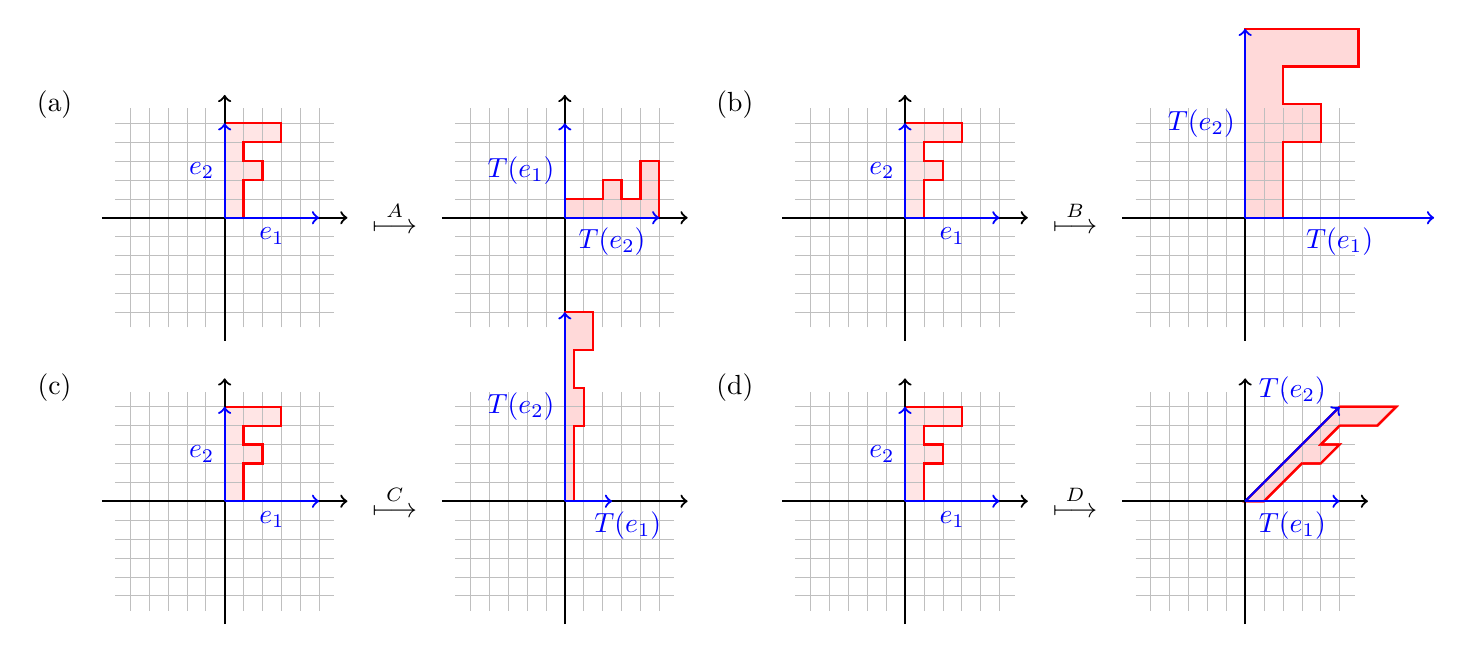
\begin{tikzpicture}[scale=0.96]
      \begin{scope}
        \path (-2.25,1.5) node {(a)};
        \begin{scope}[scale=0.25]
          \draw[red,thick,fill=red!10]
          (0,0) -- (0,5) -- (3,5) -- (3,4) -- (1,4) --
          (1,3) -- (2,3) -- (2,2) -- (1,2) -- (1,0) -- cycle;
          \draw[step=1cm, gray!50, very thin] (-5.8,-5.8) grid (5.8,5.8);
          \draw[red,thick]
          (0,0) -- (0,5) -- (3,5) -- (3,4) -- (1,4) --
          (1,3) -- (2,3) -- (2,2) -- (1,2) -- (1,0) -- cycle;
          \draw[thick,->] (-6.5,0) -- (6.5,0);
          \draw[thick,->] (0,-6.5) -- (0,6.5);
          \draw[blue,thick,->] (0,0) -- node[below] {$\vect{e}_1$} (5,0);
          \draw[blue,thick,->] (0,0) -- node[left] {$\vect{e}_2$} (0,5);
        \end{scope}
        \begin{scope}[xshift=2.25cm]
          \path (0,0) node {$\stackrel{A}{\longmapsto}$};
        \end{scope}
        \begin{scope}[xshift=4.5cm,scale=0.25]
          \draw[red,thick,fill=red!15,cm={0,1,1,0,(0,0)}]
          (0,0) -- (0,5) -- (3,5) -- (3,4) -- (1,4) --
          (1,3) -- (2,3) -- (2,2) -- (1,2) -- (1,0) -- cycle;
          \draw[step=1cm, gray!50, very thin] (-5.8,-5.8) grid (5.8,5.8);
          \draw[red,thick,cm={0,1,1,0,(0,0)}]
          (0,0) -- (0,5) -- (3,5) -- (3,4) -- (1,4) --
          (1,3) -- (2,3) -- (2,2) -- (1,2) -- (1,0) -- cycle;
          \draw[thick,->] (-6.5,0) -- (6.5,0);
          \draw[thick,->] (0,-6.5) -- (0,6.5);
          \draw[blue,thick,->,cm={0,1,1,0,(0,0)}] (0,0) -- 
          node[left] {$T(\vect{e}_1)$} (5,0);
          \draw[blue,thick,->,cm={0,1,1,0,(0,0)}] (0,0) -- 
          node[below] {$T(\vect{e}_2)$} (0,5);
        \end{scope}
      \end{scope}
      \begin{scope}[xshift=9cm]
        \path (-2.25,1.5) node {(b)};
        \begin{scope}[scale=0.25]
          \draw[red,thick,fill=red!10]
          (0,0) -- (0,5) -- (3,5) -- (3,4) -- (1,4) --
          (1,3) -- (2,3) -- (2,2) -- (1,2) -- (1,0) -- cycle;
          \draw[step=1cm, gray!50, very thin] (-5.8,-5.8) grid (5.8,5.8);
          \draw[red,thick]
          (0,0) -- (0,5) -- (3,5) -- (3,4) -- (1,4) --
          (1,3) -- (2,3) -- (2,2) -- (1,2) -- (1,0) -- cycle;
          \draw[thick,->] (-6.5,0) -- (6.5,0);
          \draw[thick,->] (0,-6.5) -- (0,6.5);
          \draw[blue,thick,->] (0,0) -- node[below] {$\vect{e}_1$} (5,0);
          \draw[blue,thick,->] (0,0) -- node[left] {$\vect{e}_2$} (0,5);
        \end{scope}
        \begin{scope}[xshift=2.25cm]
          \path (0,0) node {$\stackrel{B}{\longmapsto}$};
        \end{scope}
        \begin{scope}[xshift=4.5cm,scale=0.25]
          \draw[red,thick,fill=red!15,cm={2,0,0,2,(0,0)}]
          (0,0) -- (0,5) -- (3,5) -- (3,4) -- (1,4) --
          (1,3) -- (2,3) -- (2,2) -- (1,2) -- (1,0) -- cycle;
          \draw[step=1cm, gray!50, very thin] (-5.8,-5.8) grid (5.8,5.8);
          \draw[red,thick,cm={2,0,0,2,(0,0)}]
          (0,0) -- (0,5) -- (3,5) -- (3,4) -- (1,4) --
          (1,3) -- (2,3) -- (2,2) -- (1,2) -- (1,0) -- cycle;
          \draw[thick] (-6.5,0) -- (6.5,0);
          \draw[thick] (0,-6.5) -- (0,6.5);
          \draw[blue,thick,->,cm={2,0,0,2,(0,0)}] (0,0) -- 
          node[below] {$T(\vect{e}_1)$} (5,0);
          \draw[blue,thick,->,cm={2,0,0,2,(0,0)}] (0,0) -- 
          node[left] {$T(\vect{e}_2)$} (0,5);
        \end{scope}
      \end{scope}
      \begin{scope}[yshift=-3.75cm]
        \path (-2.25,1.5) node {(c)};
        \begin{scope}[scale=0.25]
          \draw[red,thick,fill=red!10]
          (0,0) -- (0,5) -- (3,5) -- (3,4) -- (1,4) --
          (1,3) -- (2,3) -- (2,2) -- (1,2) -- (1,0) -- cycle;
          \draw[step=1cm, gray!50, very thin] (-5.8,-5.8) grid (5.8,5.8);
          \draw[red,thick]
          (0,0) -- (0,5) -- (3,5) -- (3,4) -- (1,4) --
          (1,3) -- (2,3) -- (2,2) -- (1,2) -- (1,0) -- cycle;
          \draw[thick,->] (-6.5,0) -- (6.5,0);
          \draw[thick,->] (0,-6.5) -- (0,6.5);
          \draw[blue,thick,->] (0,0) -- node[below] {$\vect{e}_1$} (5,0);
          \draw[blue,thick,->] (0,0) -- node[left] {$\vect{e}_2$} (0,5);
        \end{scope}
        \begin{scope}[xshift=2.25cm]
          \path (0,0) node {$\stackrel{C}{\longmapsto}$};
        \end{scope}
        \begin{scope}[xshift=4.5cm,scale=0.25]
          \draw[red,thick,fill=red!15,cm={0.5,0,0,2,(0,0)}]
          (0,0) -- (0,5) -- (3,5) -- (3,4) -- (1,4) --
          (1,3) -- (2,3) -- (2,2) -- (1,2) -- (1,0) -- cycle;
          \draw[step=1cm, gray!50, very thin] (-5.8,-5.8) grid (5.8,5.8);
          \draw[red,thick,cm={0.5,0,0,2,(0,0)}]
          (0,0) -- (0,5) -- (3,5) -- (3,4) -- (1,4) --
          (1,3) -- (2,3) -- (2,2) -- (1,2) -- (1,0) -- cycle;
          \draw[thick,->] (-6.5,0) -- (6.5,0);
          \draw[thick] (0,-6.5) -- (0,6.5);
          \draw[blue,thick,->,cm={0.5,0,0,2,(0,0)}] (0,0) -- 
          node[below,xshift=0.5cm] {$T(\vect{e}_1)$} (5,0);
          \draw[blue,thick,->,cm={0.5,0,0,2,(0,0)}] (0,0) -- 
          node[left] {$T(\vect{e}_2)$} (0,5);
        \end{scope}
      \end{scope}
      \begin{scope}[xshift=9cm,yshift=-3.75cm]
        \path (-2.25,1.5) node {(d)};
        \begin{scope}[scale=0.25]
          \draw[red,thick,fill=red!10]
          (0,0) -- (0,5) -- (3,5) -- (3,4) -- (1,4) --
          (1,3) -- (2,3) -- (2,2) -- (1,2) -- (1,0) -- cycle;
          \draw[step=1cm, gray!50, very thin] (-5.8,-5.8) grid (5.8,5.8);
          \draw[red,thick]
          (0,0) -- (0,5) -- (3,5) -- (3,4) -- (1,4) --
          (1,3) -- (2,3) -- (2,2) -- (1,2) -- (1,0) -- cycle;
          \draw[thick,->] (-6.5,0) -- (6.5,0);
          \draw[thick,->] (0,-6.5) -- (0,6.5);
          \draw[blue,thick,->] (0,0) -- node[below] {$\vect{e}_1$} (5,0);
          \draw[blue,thick,->] (0,0) -- node[left] {$\vect{e}_2$} (0,5);
        \end{scope}
        \begin{scope}[xshift=2.25cm]
          \path (0,0) node {$\stackrel{D}{\longmapsto}$};
        \end{scope}
        \begin{scope}[xshift=4.5cm,scale=0.25]
          \draw[red,thick,fill=red!15,cm={1,0,1,1,(0,0)}]
          (0,0) -- (0,5) -- (3,5) -- (3,4) -- (1,4) --
          (1,3) -- (2,3) -- (2,2) -- (1,2) -- (1,0) -- cycle;
          \draw[step=1cm, gray!50, very thin] (-5.8,-5.8) grid (5.8,5.8);
          \draw[red,thick,cm={1,0,1,1,(0,0)}]
          (0,0) -- (0,5) -- (3,5) -- (3,4) -- (1,4) --
          (1,3) -- (2,3) -- (2,2) -- (1,2) -- (1,0) -- cycle;
          \draw[thick,->] (-6.5,0) -- (6.5,0);
          \draw[thick,->] (0,-6.5) -- (0,6.5);
          \draw[blue,thick,->,cm={1,0,1,1,(0,0)}] (0,0) -- 
          node[below] {$T(\vect{e}_1)$} (5,0);
          \draw[blue,thick,->,cm={1,0,1,1,(0,0)}] (0,0) -- 
          node[above,yshift=0.5cm] {$T(\vect{e}_2)$} (0,5);
        \end{scope}
      \end{scope}
    \end{tikzpicture}
  \end{center}
  The transformation $A$ is a reflection%
  \index{matrix!of a reflection}%
  \index{reflection!matrix of}%
  \index{linear transformation!reflection} about the line $x=y$. The
  transformation $B$ is a scaling%
  \index{matrix!of a scaling}%
  \index{scaling!matrix of}%
  \index{linear transformation!scaling} by a factor of $2$. The
  transformation $C$ is also a scaling, but by a different factor in
  the $x$- and $y$-directions. It scales the $x$-direction by a factor
  of $\frac{1}{2}$ (or equivalently, shrinks it by a factor of $2$),
  and scales the $y$-direction by a factor of $2$. The transformation
  $D$ is called a \textbf{shearing}%
  \index{matrix!of a shearing}%
  \index{shearing!matrix of}%
  \index{linear transformation!shearing}.
\end{solution}

\begin{example}{Rotation in $\R^3$}{rotation-R3}
  Find the matrix of a rotation%
  \index{matrix!of a rotation}%
  \index{rotation!matrix of}%
  \index{linear transformation!rotation} by angle $\theta$ about the
  $z$-axis in $3$-dimensional space, counterclockwise when viewed from
  above.
\end{example}

\begin{solution}
  Here is the before-and-after picture. A rotation in $3$-dimensional
  space is usually harder to visualize than in the plane, but
  fortunately, the rotation is about the $z$-axis, so all the
  ``action'' is taking place in the $xy$-plane.
  \begin{center}
    \begin{tikzpicture}
      \begin{scope}[scale=0.5]
        \begin{scope}[cm={-0.4,-0.5,1,0,(0,0)}]
          \draw[red,thick,fill=red!10]
          (0,0) -- (0,5) -- (3,5) -- (3,4) -- (1,4) --
          (1,3) -- (2,3) -- (2,2) -- (1,2) -- (1,0) -- cycle;
          \draw[gray!50, very thin] (0,0) circle [radius=5cm];
          \draw[red,thick]
          (0,0) -- (0,5) -- (3,5) -- (3,4) -- (1,4) --
          (1,3) -- (2,3) -- (2,2) -- (1,2) -- (1,0) -- cycle;
          \draw[thick,->] (-6.5,0) -- (6.5,0);
          \draw[thick,->] (0,-6.5) -- (0,6.5);
          \draw[blue,thick,->] (0,0) -- node[left] {$\vect{e}_1$} (5,0);
          \draw[blue,thick,->] (0,0) -- node[above] {$\vect{e}_2$} (0,5);
        \end{scope}
        \draw[thick,->] (0,0) -- (0,6.5);
        \draw[blue,thick,->] (0,0) -- node[left] {$\vect{e}_3$} (0,5);
      \end{scope}
      \begin{scope}[xshift=4.5cm]
        \path (0,0) node {$\stackrel{T}{\longmapsto}$};
      \end{scope}
      \begin{scope}[xshift=9cm,scale=0.5]
        \begin{scope}[cm={-0.4,-0.5,1,0,(0,0)}]
          \draw[red,thick,fill=red!15,rotate=30]
          (0,0) -- (0,5) -- (3,5) -- (3,4) -- (1,4) --
          (1,3) -- (2,3) -- (2,2) -- (1,2) -- (1,0) -- cycle;
          \filldraw[fill=green!20,draw=green!50!black] (0,0) -- (0:30mm) arc (0:30:30mm) -- cycle;
          \node at (15:20mm){$\theta$};
          \draw[gray!50, very thin] (0,0) circle [radius=5cm];
          \draw[red,thick,rotate=30]
          (0,0) -- (0,5) -- (3,5) -- (3,4) -- (1,4) --
          (1,3) -- (2,3) -- (2,2) -- (1,2) -- (1,0) -- cycle;
          \draw[thick,->] (-6.5,0) -- (6.5,0);
          \draw[thick,->] (0,-6.5) -- (0,6.5);
          \draw[blue,thick,->,rotate=30] (0,0) -- (5,0) node[below,xshift=1cm]
          {$T(\vect{e}_1) = \begin{mysmallmatrix}{c}\cos\theta\\\sin\theta\\0\end{mysmallmatrix}$};
          \draw[blue,thick,->,rotate=30] (0,0) -- (0,5)
          node[above,xshift=1cm] {$T(\vect{e}_2) = \begin{mysmallmatrix}{c}-\sin\theta\\\cos\theta\\0\end{mysmallmatrix}$};
        \end{scope}
        \draw[thick,->] (0,0) -- (0,6.5);
        \draw[blue,thick,->] (0,0) -- node[left] {$T(\vect{e}_3)=\begin{mysmallmatrix}{c}0\\0\\1\end{mysmallmatrix}$} (0,5);
      \end{scope}
    \end{tikzpicture}
  \end{center}
  Therefore, the matrix of the rotation is
  \begin{equation*}
    A = \begin{mymatrix}{ccc}
      \cos\theta & -\sin\theta & 0 \\
      \sin\theta & \cos\theta & 0 \\
      0 & 0 & 1
    \end{mymatrix}.
  \end{equation*}
\end{solution}

